\section{Initialization and numerical repair on CIFAR-10}
\label{supp:cifar}

\subsection{Checkpoint, references, and evaluation units}
The checkpoint is \texttt{google/ddpm-cifar10-32}, revision
\texttt{267b167dc01f0e4e6192\allowbreak{}3ea244e8b988f84deb80}. We retain its standard
epsilon prediction, variance schedule, and clipping configuration.
DINOv2-base~\cite{oquab2024dinov2} uses revision
\texttt{f9e44c814b77203eaa57\allowbreak{}a6bdbbd535f21ede1415}; Inception uses the standard
\texttt{pytorch-fid} weights. Features are deterministic. DINO inputs are
bilinearly resized to $224\times224$, normalized with ImageNet mean and
standard deviation, and represented by the final CLS token. The cached
teacher features use the identical preprocessing.

Teacher images 0--4,999 fit PCA, regions, initial moments, and support geometry;
5,000--9,999 calibrate tails; 10,000--19,999 evaluate. The real reference is
the 10,000-image CIFAR-10 test split. Reusing these fixed benchmark references
from pilot to final evaluation means that the held-out component is the
generated seed set, not previously unseen real data. Each panel uses disjoint,
equally sized teacher and real-reference rows. All arms within a study share
generated seeds and reference panels. No bootstrap duplicates enter nearest
neighbor metrics or KID. Uncertainty is conditional on the fixed benchmark
references and summarizes five independent generated panels.

Global variance ratios use the first 128 unwhitened teacher-fit PCA coordinates
in pixels and DINO features. Regional spread uses 32 unwhitened PCA coordinates;
region assignments and support distances use their whitened coordinates.
PRDC~\cite{naeem2020density} uses $k=5$ and all 768 DINO coordinates. KID~\cite{binkowski2018demystifying} is the
unbiased degree-three polynomial-kernel statistic on 2,048-dimensional standard
Inception features, computed over each full panel in float64. FID~\cite{heusel2017gans} is computed
on all 10,000 generated and 10,000 real samples; it is reported without a
confidence interval. Means and 95\% Student-$t$ intervals use the five panels;
contrasts pair the same panels. These intervals do not quantify uncertainty
over checkpoints, datasets, or unseen prompt populations.

\subsection{Frozen studies and executable interventions}
The development seed range begins at 160010, the original final range at 260010,
the trajectory control at 360010, the reference check at 460010, and independent
initializer confirmation at 660010. A separate generator per image makes the
noise seed independent of batching. Timestamped protocols and amendments were
written before their corresponding final outcomes. The 22-arm primary study
includes leading/trailing DDIM, stochastic trailing DDIM with $\eta=1$,
DPM++2M, UniPC, initial-moment correction, and output-moment correction.
The two-step DPM++/UniPC comparisons were added before their final measurements.
The CAS comparison, mean/covariance ablation, and fresh covariance-only
confirmation are separate recorded studies. Every arm is retained below.

At $K=2,4,8$ denoiser calls, trailing DDIM, DPM++2M, and UniPC use identical timestep grids,
for example $[999,749,499,249]$ at four steps. Leading grids start at 500,750,
and 875 respectively and therefore change both initialization and integration
when the budget changes. Official scheduler prediction transforms and clipping
are retained; practical solver differences are not attributed solely to order.

Let $U\in\mathbb R^{3072\times128}$ contain 128 orthonormal teacher-fit
pixel components and $\widehat\lambda\in\mathbb R^{128}$ their sample
variances. Let $I$ be the pixel-space identity and
$\widehat\sigma^2_\perp$ the remaining variance divided by $3072-128$.
The clean covariance estimate is
\begin{equation}
\widehat C=U\operatorname{diag}(\widehat\lambda)U^\top
+\widehat\sigma^2_\perp(I-UU^\top),
\label{eq:supp_cifar_covariance}
\end{equation}
For standard Gaussian noise $Z\sim\mathcal N(0,I)$, the centered remedy initializes
$[(1-\bar\alpha_{\rm start})I+\bar\alpha_{\rm start}\widehat C]^{1/2}Z$,
where $\bar\alpha_{\rm start}$ is the cumulative signal coefficient at the first timestep.
The full-moment variant additionally adds
$\sqrt{\bar\alpha_{\rm start}}\widehat\mu$, where $\widehat\mu$ is the
teacher-fit pixel mean. The mean-only ablation adds this term to unscaled
$Z$. None requires an additional denoiser call.

Output restoration fits a Gaussian Bures map in 64 teacher-fit pixel PCA
coordinates using only the pilot leading-DDIM outputs. If $C_s,C_r$ are
their source and reference covariances, the map is
$A=C_s^{-1/2}(C_s^{1/2}C_rC_s^{1/2})^{1/2}C_s^{-1/2}$.
It maps projected means and covariances, preserves the orthogonal residual,
and clips final pixels to the valid range. Map parameters are frozen before
final evaluation. It adds no denoiser calls; clipping affects approximately
3.0\% of pixel coordinates at four steps. At four calls, this control raises the pixel variance ratio from 0.376 to
0.917 while lowering real-data coverage from 0.478 to 0.332 and worsening
KID from 0.0903 to 0.1024. UniPC at the same four-call budget reaches
coverage 0.549 and KID 0.0694. The outcome comparison separates restored
pixel spread from improved fidelity and coverage.

% BEGIN AUTO ALLARMS
\begin{table*}[t]
\centering
\small
\setlength{\tabcolsep}{3.5pt}
\caption{Complete original primary (P), CAS (C), and initializer-ablation (A) comparisons, each with 10,000 generated images. VR is teacher-relative variance ratio; precision/coverage use real-data DINO features. KID intervals summarize five 2,000-image panels. Calls count forwards plus JVPs for CAS (3/7 within 4/8 ceilings). Bures reuses the corresponding DDIM outputs; its denoiser cost is that source cost and its extra transformation time is not recorded. Wall time is shared-device generation time in seconds. Full intervals for every metric are in the machine-readable results.}
\label{tab:cifar_allarms}
\begin{tabular}{llrrrrrrr}
\toprule
Method & Calls & FID$\downarrow$ & Pixel VR & DINO VR & Prec.$\uparrow$ & Cov.$\uparrow$ & KID$\times10^3\downarrow$ & Sec. \\
\midrule
P: Initial mean+cov. & 1 & 285.0 & 0.929 & 0.128 & 0.938 & 0.091 & $306.8\pm1.8$ & 3.3 \\
P: DDIM leading & 1 & 450.9 & 0.109 & 0.016 & 0.001 & 0.000 & $585.5\pm3.3$ & 7.5 \\
P: DDIM trailing & 1 & 319.9 & 0.250 & 0.083 & 0.552 & 0.022 & $347.6\pm1.1$ & 3.7 \\
A: Initial cov. & 2 & 138.8 & 0.653 & 0.411 & 0.968 & 0.298 & $126.1\pm2.1$ & 20.4 \\
A: Initial mean & 2 & 188.4 & 0.106 & 0.296 & 0.960 & 0.205 & $205.4\pm1.7$ & 27.4 \\
P: DPM++2M & 2 & 242.8 & 0.266 & 0.283 & 0.608 & 0.108 & $223.2\pm2.9$ & 17.4 \\
P: Initial mean+cov. & 2 & 146.4 & 0.631 & 0.422 & 0.963 & 0.297 & $141.3\pm2.2$ & 7.1 \\
P: DDIM leading & 2 & 182.2 & 0.109 & 0.281 & 0.969 & 0.203 & $185.3\pm1.8$ & 7.1 \\
P: DDIM trailing & 2 & 216.3 & 0.198 & 0.288 & 0.797 & 0.131 & $192.2\pm2.6$ & 7.1 \\
P: UniPC & 2 & 242.8 & 0.266 & 0.283 & 0.608 & 0.108 & $223.2\pm2.9$ & 15.2 \\
C: CAS & 3 & 282.7 & 0.357 & 0.130 & 0.788 & 0.077 & $290.2\pm3.2$ & 107.1 \\
P: Output Bures & 4 & 111.1 & 0.917 & 0.515 & 0.966 & 0.332 & $102.4\pm1.6$ & --- \\
P: DPM++2M & 4 & 80.1 & 0.599 & 0.733 & 0.918 & 0.526 & $77.4\pm2.7$ & 11.7 \\
P: DDIM $\eta=1$ & 4 & 149.1 & 0.207 & 0.547 & 0.911 & 0.327 & $161.6\pm4.4$ & 14.1 \\
P: Initial mean+cov. & 4 & 89.7 & 0.473 & 0.686 & 0.932 & 0.488 & $92.6\pm2.4$ & 13.7 \\
P: DDIM leading & 4 & 87.9 & 0.376 & 0.677 & 0.935 & 0.478 & $90.3\pm2.5$ & 13.9 \\
P: DDIM trailing & 4 & 111.2 & 0.371 & 0.638 & 0.911 & 0.428 & $113.2\pm4.2$ & 12.1 \\
P: UniPC & 4 & 73.1 & 0.671 & 0.758 & 0.913 & 0.549 & $69.4\pm2.6$ & 13.6 \\
C: CAS & 7 & 217.3 & 0.661 & 0.309 & 0.961 & 0.227 & $243.3\pm5.5$ & 220.9 \\
P: Output Bures & 8 & 56.4 & 0.949 & 0.812 & 0.927 & 0.596 & $50.5\pm1.8$ & --- \\
P: DPM++2M & 8 & 32.5 & 0.943 & 0.975 & 0.859 & 0.731 & $26.4\pm1.2$ & 23.7 \\
P: DDIM $\eta=1$ & 8 & 74.3 & 0.387 & 0.825 & 0.906 & 0.564 & $71.2\pm2.9$ & 36.2 \\
P: Initial mean+cov. & 8 & 42.6 & 0.633 & 0.913 & 0.892 & 0.676 & $37.8\pm2.2$ & 41.5 \\
P: DDIM leading & 8 & 41.0 & 0.624 & 0.915 & 0.893 & 0.680 & $36.3\pm2.1$ & 24.5 \\
P: DDIM trailing & 8 & 48.3 & 0.606 & 0.903 & 0.879 & 0.649 & $43.5\pm2.3$ & 25.7 \\
P: UniPC & 8 & 31.3 & 1.020 & 0.986 & 0.849 & 0.740 & $24.5\pm1.1$ & 34.5 \\
\bottomrule
\end{tabular}
\end{table*}
% END AUTO ALLARMS

\subsection{Covariance initialization improves two-call fidelity and coverage}
\label{supp:cifar_initializer}
Covariance-only initialization reduces two-call KID from 0.1858 to 0.1264
(32.0\%) in the separate fresh confirmation, while real-data DINO coverage
increases from 0.206 to 0.288. These are five paired generated panels from
one fixed pretrained checkpoint. The earlier secondary ablation isolates
mean and covariance using the original paired seeds: its KID values are
0.1261 for covariance, 0.1413 for full moments, and 0.2054 for mean only.
That analysis motivated the separately predeclared fresh-sample study;
the original frozen selector and all earlier outcomes remain unchanged. The primary confirmation
criterion is lower real-data KID against each of the five declared alternatives;
all other metrics remain reported. Table~\ref{tab:cifar_v2_contrasts} gives
complete paired contrasts and simultaneous intervals. Coverage is similar
between the two covariance variants, so the mean-term finding concerns KID,
not an improvement in every metric.

% BEGIN AUTO V2CONTRASTS
\begin{table*}[t]
\centering
\small
\setlength{\tabcolsep}{3.5pt}
\caption{All five prespecified fresh-confirmation contrasts: centered covariance initializer minus comparator. KID intervals simultaneously cover the five comparisons at 95\% by Bonferroni adjustment; coverage intervals are ordinary paired 95\% intervals. Negative KID and positive coverage differences favor the centered initializer.}
\label{tab:cifar_v2_contrasts}
\begin{tabular}{lrrrr}
\toprule
Comparator & $\Delta$KID$\times10^3$ & Simultaneous interval & $\Delta$coverage & Paired interval \\
\midrule
DDIM leading & -59.38 & [-61.38,-57.39] & 0.0821 & [0.0672,0.0970] \\
DDIM trailing & -65.90 & [-70.11,-61.69] & 0.1575 & [0.1501,0.1649] \\
DPM++2M & -96.14 & [-100.61,-91.66] & 0.1820 & [0.1714,0.1926] \\
UniPC & -96.14 & [-100.61,-91.66] & 0.1820 & [0.1714,0.1926] \\
Initial mean+cov. & -14.11 & [-17.90,-10.31] & -0.0012 & [-0.0157,0.0133] \\
\bottomrule
\end{tabular}
\end{table*}
% END AUTO V2CONTRASTS

\begin{figure}[t]
\centering
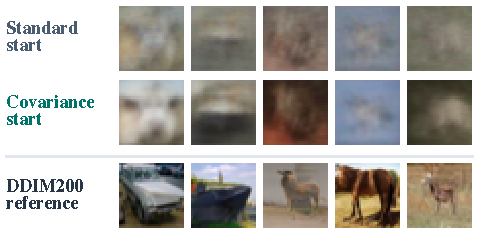
\includegraphics[width=\linewidth]{../figures/initializer_examples.pdf}
\caption{Fixed-index examples from the two-call standard-normal and
covariance-start arms. The two upper rows are paired by initial noise seed,
using the eighth image of each saved 2,000-image panel. The separately
seeded DDIM200 row uses the eighth image of each 400-image reference
panel and provides a visual reference. Every selected image is displayed.}
\label{fig:initializer_examples}
\end{figure}

\subsection{The same outputs improve under an untouched external reference}
\label{supp:cifar101}
The unchanged covariance-initialized outputs reduce KID by 32.7\% against
untouched CIFAR-10.1v6. This separate reference evaluation was frozen
before downloading or scoring CIFAR-10.1v6~\cite{recht2018cifar10}.
The official release supplies
2,000 images, exactly 200 per class, sampled separately for testing CIFAR-10
generalization. We pin repository commit
\texttt{d9982abb0bfc4846b8d1\allowbreak{}3a11e66b887d946205d0}, preserve file hashes,
and verify shapes, class counts, and absence of exact pixel duplicates with
the original CIFAR-10 test reference. This is a new reference for our method
development; it does not assert that general-purpose pretrained representations
have never encountered related public images.

Every available 10,000-image confirmatory candidate is included: 22 primary
arms, two CAS arms, two initializer ablations, and six fresh initializer arms.
Generated images, seeds, features, methods, and selections remain unchanged.
The same frozen Inception and DINO extraction pipeline embeds the new real
reference. Each arm's five disjoint 2,000-image generated panels is compared
to all 2,000 external reference images. Consequently, Student-$t$ intervals
condition on this shared real reference. Four prespecified paired KID contrasts
receive Bonferroni 98.75\% marginal intervals, giving simultaneous 95\%
coverage for that four-comparison family under the panel-effect approximation.
Precision and coverage intervals are descriptive. We do not use bootstrapped
image duplicates in nearest-neighbor metrics.

All four predicted KID directions hold (Fig.~\ref{fig:cifar101}). Output
covariance restoration at four calls worsens KID by 0.01070 [0.00843,0.01297]
and decreases coverage by 0.1269, despite increasing precision by 0.0262.
UniPC4 improves KID by 0.02182 [0.02015,0.02348] and coverage by 0.0564,
with a 0.0228 precision decrease. In the fresh two-call confirmation,
centered initialization reduces KID from 0.19060 to 0.12832, a 32.7\%
reduction; its paired difference is $-0.06228$ [$-0.06422,-0.06035$].
Coverage rises from 0.3221 to 0.4268 (difference 0.1047 [0.0895,0.1199]),
while precision decreases from 0.9756 to 0.9580. Compared with mean-plus-covariance
initialization, centered initialization improves KID by 0.01272
[0.00896,0.01647]; its coverage difference is $-0.0072$
[$-0.0198,0.0054$]. Thus the external reference supports both the useful
initialization repair and the failure of output-moment restoration, while
retaining the observed fidelity--coverage tradeoffs.

No additional denoiser samples are generated. DINO and Inception extraction
of the 2,000 new images takes 8.6 and 53.0 recorded seconds on shared hardware;
all 32-arm metric evaluation takes 9.4 seconds. The artifact manifest records
reference and feature hashes, the frozen protocol, source hashes, resource
use, and every primary comparison. Table~\ref{tab:cifar101_all} retains every
arm, including unfavorable CAS and initializer comparisons.

\begin{figure*}[t]
\centering
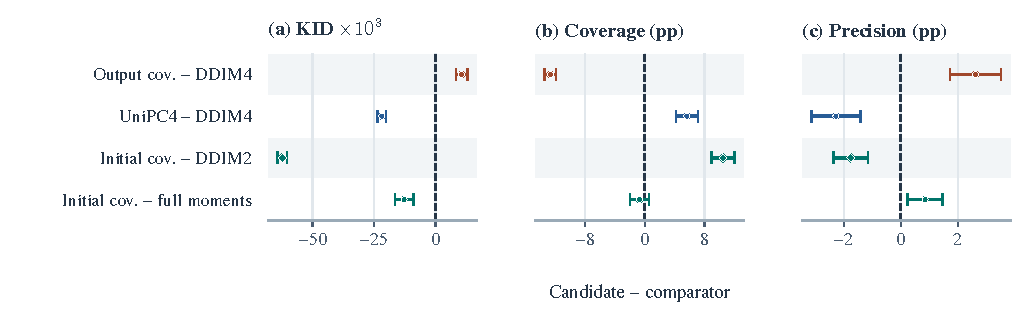
\includegraphics[width=\textwidth]{../figures/cifar101_confirmation.pdf}
\caption{Untouched CIFAR-10.1v6 confirmation using unchanged generated samples.
Four prespecified contrasts are shown. KID intervals have the four-comparison
adjustment; coverage and precision use ordinary 95\% intervals. All intervals
condition on the fixed external real reference. Opposing precision and
coverage changes reinforce the need for multiple measurements.}
\label{fig:cifar101}
\end{figure*}
\begin{table*}[t]
\centering\footnotesize
\setlength{\tabcolsep}{4pt}
\caption{Untouched CIFAR-10.1v6 reference evaluation. All 32 frozen candidate arms are retained. Mean $\pm$95\% interval over five independent generated panels, conditional on the same fixed 2,000-image external reference. DINO precision and coverage are descriptive. P/C/A/V2 denote primary/CAS/initializer ablation/fresh initializer confirmation.}
\label{tab:cifar101_all}
\begin{tabular}{llrrr}
\toprule
Study & Arm & KID$\times10^3\downarrow$ & Precision$\uparrow$ & Coverage$\uparrow$ \\
\midrule
P & Output covariance 4 & $100.825\pm0.422$ & $0.948\pm0.002$ & $0.481\pm0.005$ \\
P & Output covariance 8 & $48.546\pm0.898$ & $0.909\pm0.007$ & $0.715\pm0.014$ \\
P & DPM++ 2 & $232.929\pm3.237$ & $0.614\pm0.016$ & $0.154\pm0.024$ \\
P & DPM++ 4 & $76.362\pm1.481$ & $0.904\pm0.006$ & $0.646\pm0.014$ \\
P & DPM++ 8 & $25.346\pm0.446$ & $0.852\pm0.008$ & $0.790\pm0.010$ \\
P & Stochastic DDIM 4 & $163.798\pm2.586$ & $0.864\pm0.007$ & $0.446\pm0.024$ \\
P & Stochastic DDIM 8 & $72.596\pm2.015$ & $0.884\pm0.011$ & $0.653\pm0.012$ \\
P & Initial mean+cov. 1 & $316.809\pm1.891$ & $0.973\pm0.004$ & $0.132\pm0.007$ \\
P & Initial mean+cov. 2 & $141.748\pm1.833$ & $0.949\pm0.006$ & $0.437\pm0.014$ \\
P & Initial mean+cov. 4 & $92.056\pm1.769$ & $0.919\pm0.009$ & $0.619\pm0.012$ \\
P & Initial mean+cov. 8 & $36.878\pm0.972$ & $0.881\pm0.007$ & $0.761\pm0.016$ \\
P & Leading DDIM 1 & $595.636\pm2.339$ & $0.000\pm0.000$ & $0.000\pm0.000$ \\
P & Leading DDIM 2 & $189.848\pm2.061$ & $0.979\pm0.005$ & $0.322\pm0.020$ \\
P & Leading DDIM 4 & $90.125\pm1.802$ & $0.922\pm0.008$ & $0.608\pm0.011$ \\
P & Leading DDIM 8 & $35.464\pm1.075$ & $0.884\pm0.013$ & $0.763\pm0.015$ \\
P & Trailing DDIM 1 & $353.858\pm1.587$ & $0.390\pm0.017$ & $0.022\pm0.009$ \\
P & Trailing DDIM 2 & $199.990\pm2.138$ & $0.791\pm0.016$ & $0.195\pm0.012$ \\
P & Trailing DDIM 4 & $113.551\pm3.041$ & $0.876\pm0.007$ & $0.569\pm0.017$ \\
P & Trailing DDIM 8 & $42.641\pm1.168$ & $0.869\pm0.008$ & $0.741\pm0.018$ \\
P & UniPC 2 & $232.929\pm3.237$ & $0.614\pm0.016$ & $0.154\pm0.024$ \\
P & UniPC 4 & $68.309\pm1.436$ & $0.899\pm0.005$ & $0.665\pm0.014$ \\
P & UniPC 8 & $23.633\pm0.536$ & $0.845\pm0.014$ & $0.790\pm0.009$ \\
C & CAS ceiling 4 & $297.637\pm2.479$ & $0.753\pm0.011$ & $0.107\pm0.010$ \\
C & CAS ceiling 8 & $246.371\pm5.967$ & $0.971\pm0.005$ & $0.357\pm0.007$ \\
A & Initial covariance 2 & $127.881\pm1.205$ & $0.959\pm0.005$ & $0.433\pm0.015$ \\
A & Initial mean 2 & $207.572\pm1.883$ & $0.962\pm0.003$ & $0.331\pm0.012$ \\
V2 & DPM++ 2 & $232.202\pm1.627$ & $0.614\pm0.006$ & $0.152\pm0.010$ \\
V2 & Initial covariance 2 & $128.321\pm1.914$ & $0.958\pm0.007$ & $0.427\pm0.012$ \\
V2 & Initial mean+cov. 2 & $141.036\pm2.629$ & $0.950\pm0.004$ & $0.434\pm0.013$ \\
V2 & Leading DDIM 2 & $190.602\pm2.626$ & $0.976\pm0.002$ & $0.322\pm0.011$ \\
V2 & Trailing DDIM 2 & $200.159\pm2.041$ & $0.788\pm0.019$ & $0.188\pm0.006$ \\
V2 & UniPC 2 & $232.202\pm1.627$ & $0.614\pm0.006$ & $0.152\pm0.010$ \\
\bottomrule
\end{tabular}
\end{table*}


\subsection{Frozen selectors and threshold sensitivity}
% BEGIN AUTO SELECTORS
\begin{table}[t]
\centering
\small
\setlength{\tabcolsep}{3.5pt}
\caption{Frozen pilot choices evaluated on fresh generated panels. Metrics average budgets 2/4/8 within each panel, followed by the five-panel interval. The later centered-initializer confirmation is separate.}
\label{tab:cifar_selection}
\begin{tabular}{lcc}
\toprule
Selection rule & KID$\times10^3\downarrow$ & Coverage$\uparrow$ \\
\midrule
Default DDIM & $103.9\pm1.7$ & $0.453\pm0.016$ \\
Fixed DPM++ & $109.0\pm2.2$ & $0.455\pm0.011$ \\
Fixed UniPC & $105.7\pm2.1$ & $0.466\pm0.012$ \\
Variance only & $89.4\pm1.5$ & $0.456\pm0.010$ \\
Precision only & $94.0\pm2.0$ & $0.457\pm0.020$ \\
PRDC harmonic & $87.1\pm2.1$ & $0.481\pm0.019$ \\
Vendi & $78.4\pm1.8$ & $0.529\pm0.013$ \\
Teacher Fr\'echet & $78.4\pm1.8$ & $0.529\pm0.013$ \\
Audit (frozen v1) & $79.0\pm1.9$ & $0.526\pm0.015$ \\
\bottomrule
\end{tabular}
\end{table}
% END AUTO SELECTORS
The pilot audit first computes the Gaussian initialization penalty
$1-V_{\rm practical}/V_{\rm matched}$. Above 0.5 it selects initial-moment
correction. Otherwise it considers DPM++2M and UniPC on the matched trailing
grid, retaining candidates whose teacher precision is at least the
leading-DDIM precision minus 0.05, and maximizes teacher coverage. If neither
passes, it retains leading DDIM. These decisions are full moments at two calls,
UniPC at four, and DPM++ at eight; the later centered initializer does not
silently replace the original two-call choice.

The competing selectors maximize pixel variance, teacher precision, the harmonic
mean of teacher precision and coverage, or cosine-kernel Vendi, or minimize
teacher-DINO Fr\'echet distance. Vendi uses the entropy of the normalized
uncentered cosine-kernel spectrum. Fixed DPM++ and UniPC always choose that
solver. Every selector sees only pilot generated samples. The fixed benchmark
reference is shared. The audit evaluates a restricted diagnostic shortlist;
the results establish useful choices but not an optimal search policy or
a universal reduction in required diagnostic compute.

Sensitivity is reported without changing final selections. Initialization
penalty thresholds 0.25,0.5,0.75 all route only the two-call setting to
initialization correction. Precision-loss tolerances 0.05 and 0.10 preserve the
four/eight-call choices; 0.025 admits neither solver and retains the default.
Thus the latter margin is consequential and is disclosed. The support/HF
sensitivity grid includes quantiles 0.90,0.95,0.99 and excess margins
0.025,0.05,0.10, with all nine combinations reported and multiplicity expanded
accordingly. Both noisy one-step DDIM settings fail the HF gate throughout;
their feature-support gates alone can pass. Passing one feature or frequency
test is not a certificate of visual quality.

\subsection{Fidelity gates and remaining deficits}
The primary operational gates use the calibrated 95th-percentile tail and a
0.05 excess-probability margin. The final occupancy/support family contains
32 arm-study entries and two representations, including the independent
confirmation; the ten regions expand the occupancy family to 640 bounds sets.
The external HF family contains 32 entries. Previously derived outputs with
smaller families are preserved, and the reported conclusions use the expanded
family. The HF score is mean Fourier energy outside radius 8 in the
$32\times32$ grayscale frequency grid. It detects excess high-frequency
artifacts; a pass does not certify overall fidelity. Final real-data KID,
precision, and coverage provide additional outcome evidence, separately from
these operational tail tests.

Table~\ref{tab:cifar_gates} reports all final diagnoses. Counts refer to certified
feature-region mass depletion, not semantic class deletion. Even the successful
centered initializer retains DINO-region deficits and conditional contraction.
This is consistent with its remaining gap to the resolved reference and does
not negate the measured coverage gain. No CIFAR result establishes that a
deficit is caused uniquely by model training.

% BEGIN AUTO GATES
\begin{table*}[t]
\centering
\small
\setlength{\tabcolsep}{3.5pt}
\caption{Complete mechanism checks at the final multiplicity. D/P denote DINO/pixel representations. Depletion counts are among ten fixed feature regions. C/E denote conditional contraction/expansion; a dash means neither is certified. Support P means the calibrated excess-tail test passes, not visual quality. HF is the separate artifact-tail test. P/C/A/V2 denote primary, CAS, ablation, and fresh confirmation. CAS budget labels 4/8 correspond to 3/7 actual calls.}
\label{tab:cifar_gates}
\begin{tabular}{llcccc}
\toprule
Arm & Budget & Depleted D/P & Spread D/P & Support D/P & HF \\
\midrule
P: Initial mean+cov. & 1 & 9/0 & C/CE & P/P & Pass \\
P: DDIM leading & 1 & 9/9 & C/C & P/P & Fail \\
P: DDIM trailing & 1 & 9/8 & C/C & P/P & Fail \\
P: DPM++2M & 2 & 9/8 & C/C & P/P & Pass \\
P: Initial mean+cov. & 2 & 9/0 & C/C & P/P & Pass \\
P: DDIM leading & 2 & 9/3 & C/C & P/P & Pass \\
P: DDIM trailing & 2 & 9/7 & C/C & P/P & Pass \\
P: UniPC & 2 & 9/8 & C/C & P/P & Pass \\
P: Output Bures & 4 & 7/0 & C/--- & P/P & Pass \\
P: DPM++2M & 4 & 2/0 & C/C & P/P & Pass \\
P: DDIM $\eta=1$ & 4 & 6/6 & C/C & P/P & Pass \\
P: Initial mean+cov. & 4 & 3/0 & C/C & P/P & Pass \\
P: DDIM leading & 4 & 3/0 & C/C & P/P & Pass \\
P: DDIM trailing & 4 & 4/3 & C/C & P/P & Pass \\
P: UniPC & 4 & 1/0 & C/C & P/P & Pass \\
P: Output Bures & 8 & 1/0 & C/--- & P/P & Pass \\
P: DPM++2M & 8 & 0/0 & ---/--- & P/P & Pass \\
P: DDIM $\eta=1$ & 8 & 2/0 & C/C & P/P & Pass \\
P: Initial mean+cov. & 8 & 0/0 & C/C & P/P & Pass \\
P: DDIM leading & 8 & 0/0 & C/C & P/P & Pass \\
P: DDIM trailing & 8 & 0/0 & C/C & P/P & Pass \\
P: UniPC & 8 & 0/0 & ---/--- & P/P & Pass \\
C: CAS & 4 & 9/6 & C/C & P/P & Pass \\
C: CAS & 8 & 9/2 & C/C & P/P & Pass \\
A: Initial cov. & 2 & 9/0 & C/C & P/P & Pass \\
A: Initial mean & 2 & 9/2 & C/C & P/P & Pass \\
V2: DPM++2M & 2 & 9/8 & C/C & P/P & Pass \\
V2: Initial cov. & 2 & 9/0 & C/C & P/P & Pass \\
V2: Initial mean+cov. & 2 & 9/0 & C/C & P/P & Pass \\
V2: DDIM leading & 2 & 9/3 & C/C & P/P & Pass \\
V2: DDIM trailing & 2 & 9/7 & C/C & P/P & Pass \\
V2: UniPC & 2 & 9/8 & C/C & P/P & Pass \\
\bottomrule
\end{tabular}
\end{table*}
% END AUTO GATES

\subsection{Covariance-aware sampling comparison}
We port Appendix C of CAS~\cite{schioppa2026covariance} to the CIFAR checkpoint
using the published ConvDCT8 basis, channel-averaged covariance estimate,
variance cap $10^4$, and fixed first-step variance 0.1. Later steps use one
forward-mode Jacobian--vector product each. Two/four integration steps therefore
require two/four forward calls plus one/three JVPs: three/seven calls within
ceilings of four/eight. These rows are not labeled strictly equal-four/eight
cost. Shared-device wall time is reported separately.

Validation checks ConvDCT reconstruction (maximum absolute error
$2.4\times10^{-6}$), Gaussian Tweedie covariance scaling
($1.2\times10^{-7}$), and exact zero-covariance reduction to DDIM. Network JVP
agrees with centered finite differences to relative error $8.66\times10^{-4}$
at displacement 0.01; the full displacement sweep is saved. TF32 is disabled.
The primary port follows the published raw predicted-clean-sample formula;
only final pixels are clipped. A separately declared paired 2,048-image adapter
pilot moves checkpoint clipping inside that predictor. Raw versus clipped
KID is 0.2899 versus 0.3984 at the four-call ceiling and 0.2419 versus 0.2479
at eight. This obvious checkpoint adaptation does not rescue performance.
The full raw-port comparison remains reported. These outcomes concern transfer
to this checkpoint and small budget, not the general effectiveness of CAS.

\subsection{Reference stability and learned trajectories}
The reference check uses 2,000 fresh paired seeds for DDIM100, DDIM200, and
DPM++100, summarized in five 400-image panels. PRDC depends on panel size, so
its absolute values are not compared with the primary 2,000-image panels.
DDIM200 changes pixel variance ratio by 0.01095 [0.00678,0.01513], DINO ratio
by $-0.00715$ [$-0.01125,-0.00306$], KID by $-0.00170$
[$-0.00258,-0.00082$], and real coverage by $-0.0035$ [$-0.0247,0.0177$]
relative to DDIM100. The high-frequency ratio rises by 0.0907, showing why the
teacher's artifact distribution must not be treated as an absolute quality
standard. DPM++100 changes pixel ratio by 0.0669 but DINO ratio by only $-0.00168$
with an interval spanning zero. The large few-step contraction persists under
these reference perturbations.

For the Gaussian bridge, 200,000 oracle samples independently verify the
transfer identity across five covariance eigenvalues and both grids.
Learned ratios are evaluated in the separately fitted teacher basis. Leading
four/eight-step directional Spearman correlations are 0.938/0.894, whereas the
trailing one-step ordering is reversed. The formula excludes clipping and
noncommuting learned dynamics. Official DDIM grids whose internal previous-time
arithmetic does not match adjacent nodes are explicitly excluded from the
adjacent-node theory comparison.

Intermediate states from 2,048 independent paired seeds are projected into 64
teacher-fit pixel components. Cross-step linear regressions quantify mixing
and unexplained projected variation. Mean off-diagonal regression mixing is
0.0398/0.0202 for leading DDIM at four/eight calls and 0.0614/0.0215 for DPM++.
Corresponding unexplained fractions are 0.0100/0.0034 and 0.0133/0.0042.
These measurements test the diagonal approximation; omitted coordinates can
also cause regression residuals, so they do not identify nonlinear coupling
uniquely.

\begin{figure*}[t]
\centering
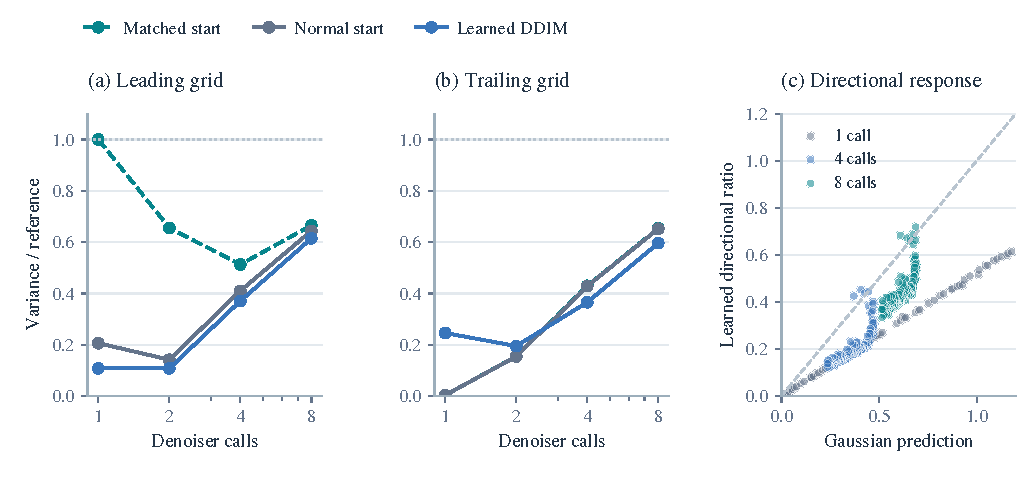
\includegraphics[width=\textwidth]{../figures/theory_initialization.pdf}
\caption{Initialization and integration in the Gaussian surrogate, with learned
CIFAR measurements in a fixed teacher-fit pixel basis. Leading spacing changes
the initial time with the budget; trailing spacing retains the noisy start.
The directional agreement at four/eight leading steps and the trailing
one-step failure delimit the empirical scope of the diagonal calculation.
These panels use the fitted reference covariance for the theory comparison;
the main benchmark metrics use independent evaluation-reference panels.}
\label{fig:cifar_theory_supp}
\end{figure*}

\begin{figure*}[t]
\centering
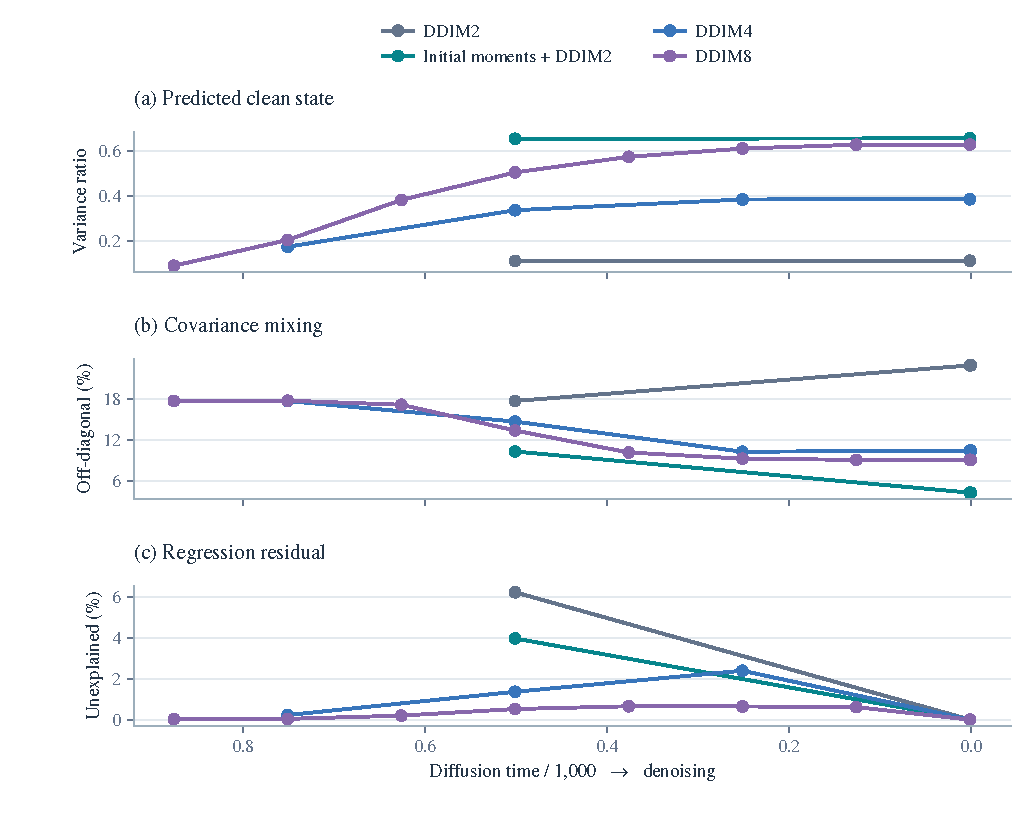
\includegraphics[width=\textwidth]{../figures/theory_trajectories.pdf}
\caption{Intermediate-state measurements in a fixed teacher-fit basis.
Estimated clean-state spread, off-diagonal covariance, and cross-step regression
residuals reveal departures from an exactly diagonal Gaussian evolution.
Projection residuals are descriptive and can include omitted-coordinate effects.}
\label{fig:cifar_trajectory_supp}
\end{figure*}

\subsection{Compute and reproducibility}
All sampling uses one H200 with float32 and at most eight CPU threads per
process. Per-arm records preserve seeds, timesteps, configuration, wall time,
peak memory, sample hashes, and source hashes. Timing reflects shared hardware
and is not a dedicated-device throughput benchmark. The complete CIFAR record
contains 403,824 images including pilot and derived-output images, and 2,256,112
denoiser-plus-JVP calls excluding reused Bures outputs and the supplied teacher.
Recorded sampling wall time totals 1,685 seconds; feature extraction and
diagnosis are additional. The primary 22-arm diagnostic takes about 60 seconds
on eight CPU threads after feature extraction, with all reference fitting
included. Frozen fits can be reused in subsequent audits.

Preparation is not free. The supplied 20,000-image DDIM100 reference represents
\textbf{2,000,000 forward-image calls}; we reuse this valid cache and do not
reconstruct its original generation wall time. The primary 22-arm pilot contains
45,056 images (22$\times$2,048), including two derived Bures outputs, and
174,080 additional denoiser calls. Its recorded generation time is 58.6 seconds;
DINO and Inception extraction records add 89.8 and 91.4 seconds. The broader
26-arm development record in Table~\ref{tab:cifar_resources} also includes four
earlier unmatched-grid solver arms.

The frozen audit's decision uses the reference-based initialization penalty at
two calls and leading-DDIM, DPM++, and UniPC pilot measurements at four/eight
calls. Those six metric inputs comprise 12,288 images and 73,728 denoiser calls;
including the two-call default and selected-remedy validation gives 16,384
images and 81,920 calls. These are input requirements of the frozen rule,
not realized savings: development actually evaluated the complete pilot.
Covariance-fit and per-image transformation wall times were not separately
recorded. ``No extra denoiser calls'' for the initializer refers only to
online sampling after preparation, not to free reference construction,
feature computation, or matrix operations. Original cached teacher-DINO
extraction time is likewise unavailable; its recorded reuse time is not
represented as extraction throughput.

The reproduction guide lists exact commands for feature extraction, generation,
metrics, diagnostics, plots, and independent confirmation. Raw outputs remain
immutable; the manifest verifies their hashes against generation records.
Editable PDF/SVG figures are generated from saved result files.
Figure~\ref{fig:initializer_examples} uses indices 7, 2007, 4007, 6007,
and 8007 in both two-call arms, with no metric-based image selection. All configurations, complete
per-panel metric arrays, gate sensitivity values, and paired contrasts are
included in the accompanying package.

% BEGIN AUTO TIMING
\begin{table*}[t]
\centering
\small
\setlength{\tabcolsep}{3.5pt}
\caption{Generation resources for every CIFAR study. Image totals include derived Bures outputs; call counts exclude their reused sampling. The supplied 20,000-image teacher and feature/metric computation are excluded. Wall time is the sum of recorded arm times on shared hardware.}
\label{tab:cifar_resources}
\begin{tabular}{lrrrr}
\toprule
Study & Arms & Images & Forward+JVP calls & Seconds \\
\midrule
Development pilot & 26 & 53,248 & 223,232 & 67.2 \\
Primary final & 22 & 220,000 & 850,000 & 333.7 \\
CAS pilot & 2 & 4,096 & 20,480 & 76.2 \\
CAS final & 2 & 20,000 & 100,000 & 328.0 \\
CAS clip adapter & 2 & 4,096 & 20,480 & 36.8 \\
Initializer ablation & 2 & 20,000 & 40,000 & 47.8 \\
Fresh initializer confirmation & 6 & 60,000 & 120,000 & 43.5 \\
Reference stability & 3 & 6,000 & 800,000 & 682.5 \\
Trajectories & 8 & 16,384 & 81,920 & 69.3 \\
\bottomrule
\end{tabular}
\end{table*}
% END AUTO TIMING

